\documentclass[11pt]{article}

% useful packages
\usepackage[english]{babel}
\usepackage{amsmath}
\usepackage{amssymb}
\usepackage{wasysym}
\usepackage{mathtools}
\usepackage{floatpag}
\usepackage{cite}
\usepackage{hyperref}
\usepackage{verbatim}
\usepackage{listings}
\usepackage{xcolor}
\usepackage{graphicx}
\usepackage{caption}
\usepackage{mwe}
\usepackage{float}


% colorful listings

\lstset{language=C,%
    breaklines=true,
    keywordstyle=\color{blue},
    morekeywords=[2]{1}, keywordstyle=[2]{\color{black}},
    identifierstyle=\color{black},%
    stringstyle=\color{olive},
    commentstyle=\color{gray},%
    showstringspaces=false,%without this there will be a symbol in the places where there is a space
    numbers=left,
    numberstyle={\tiny \color{black}},% size of the numbers
    numbersep=9pt, % this defines how far the numbers are from the text
    emph=[1]{for,end,break,if},emphstyle=[1]\color{red}, %some words to emphasise
}




\begin{document}

\title{Solution to Homework 9}

\author{
   Meshach Aruoriwo Ogbor,\\
   Md Rasel}

\maketitle

\section{Exercise 9.1 - Advanced MPI}
\lstinputlisting[language=C]{ex9.c}
For compilation on Stromboli, we used the following command: \\
\verb+ mpicc -o ex9 ex9.c+
\newpage

\section{Submit Script for exercise 9.1}
\lstinputlisting[language=bash]{job_ex9.sh}
\section{Results}

\begin{figure} [H]
   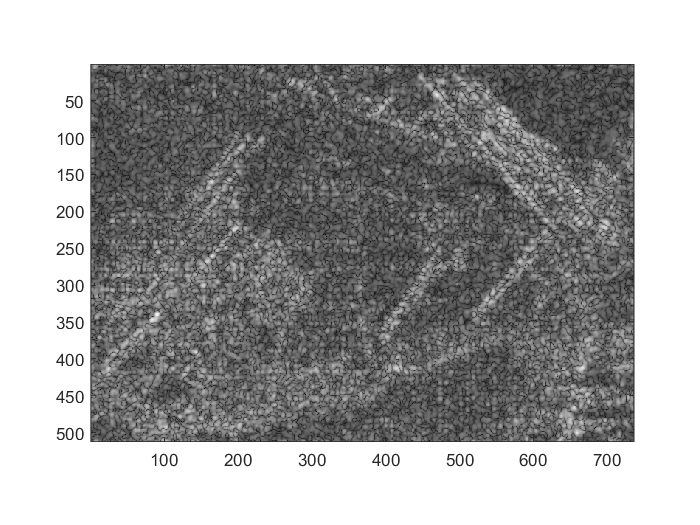
\includegraphics[width=\linewidth]{output_5.png}
   \caption{Image of iteration=5 }\label{fig1}
\end{figure}

\begin{figure} [H]
   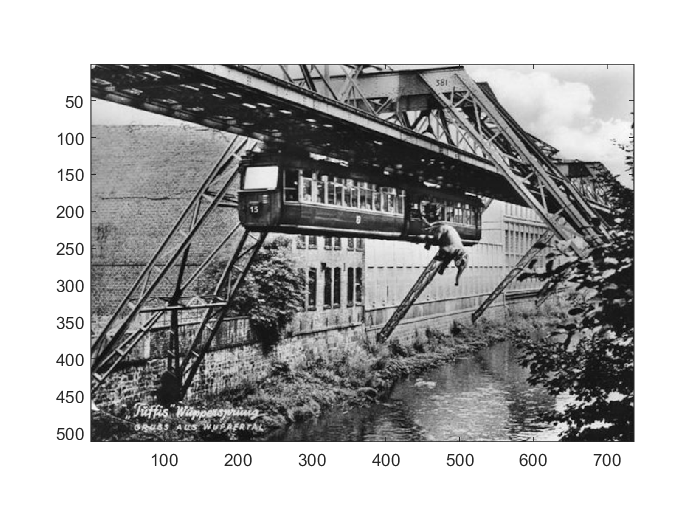
\includegraphics[width=\linewidth]{output_20.png}
   \caption{Image of iteration=20 }\label{fig1}
\end{figure}

\begin{figure} [H]
   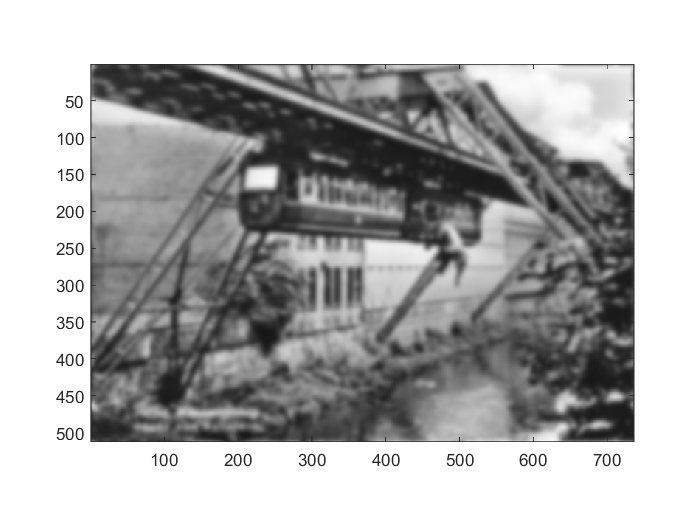
\includegraphics[width=\linewidth]{output_100.png}
   \caption{Image of iteration=100 }\label{fig1}
\end{figure}

\end{document}
